% ****** Start of file apssamp.tex ******
%
%   This file is part of the APS files in the REVTeX 4.2 distribution.
%   Version 4.2a of REVTeX, December 2014
%
%   Copyright (c) 2014 The American Physical Society.
%
%   See the REVTeX 4 README file for restrictions and more information.
%
% TeX'ing this file requires that you have AMS-LaTeX 2.0 installed
% as well as the rest of the prerequisites for REVTeX 4.2
%
% See the REVTeX 4 README file
% It also requires running BibTeX. The commands are as follows:
%
%  1)  latex apssamp.tex
%  2)  bibtex apssamp
%  3)  latex apssamp.tex
%  4)  latex apssamp.tex
%
\documentclass[%
 reprint,
%superscriptaddress,
%groupedaddress,
%unsortedaddress,
%runinaddress,
%frontmatterverbose, 
%preprint,
%preprintnumbers,
%nofootinbib,
%nobibnotes,
%bibnotes,
 amsmath,amssymb,
 aps,
%pra,
%prb,
%rmp,
%prstab,
%prstper,
%floatfix,
]{revtex4-2}

\usepackage{graphicx}% Include figure files
\usepackage{dcolumn}% Align table columns on decimal point
\usepackage{bm}% bold math
%\usepackage{hyperref}% add hypertext capabilities
%\usepackage[mathlines]{lineno}% Enable numbering of text and display math
%\linenumbers\relax % Commence numbering lines

%\usepackage[showframe,%Uncomment any one of the following lines to test 
%%scale=0.7, marginratio={1:1, 2:3}, ignoreall,% default settings
%%text={7in,10in},centering,
%%margin=1.5in,
%%total={6.5in,8.75in}, top=1.2in, left=0.9in, includefoot,
%%height=10in,a5paper,hmargin={3cm,0.8in},
%]{geometry}

\begin{document}

\preprint{APS/123-QED}

\title{Manuscript Title:\\with Forced Linebreak}% Force line breaks with \\
\thanks{A footnote to the article title}%

\author{Ann Author}
 \altaffiliation[Also at ]{Physics Department, XYZ University.}%Lines break automatically or can be forced with \\
\author{Second Author}%
 \email{Second.Author@institution.edu}
\affiliation{%
 Authors' institution and/or address\\
 This line break forced with \textbackslash\textbackslash
}%

\collaboration{MUSO Collaboration}%\noaffiliation

\author{Charlie Author}
 \homepage{http://www.Second.institution.edu/~Charlie.Author}
\affiliation{
 Second institution and/or address\\
 This line break forced% with \\
}%
\affiliation{
 Third institution, the second for Charlie Author
}%
\author{Delta Author}
\affiliation{%
 Authors' institution and/or address\\
 This line break forced with \textbackslash\textbackslash
}%

\collaboration{CLEO Collaboration}%\noaffiliation

\date{\today}% It is always \today, today,
             %  but any date may be explicitly specified

\begin{abstract}
An article usually includes an abstract, a concise summary of the work
covered at length in the main body of the article. 
\begin{description}
\item[Usage]
Secondary publications and information retrieval purposes.
\item[Structure]
You may use the \texttt{description} environment to structure your abstract;
use the optional argument of the \verb+\item+ command to give the category of each item. 
\end{description}
\end{abstract}

%\keywords{Suggested keywords}%Use showkeys class option if keyword
                              %display desired
\maketitle

%\tableofcontents

\section{\label{sec:level1}  Introduction}
\section{\label{sec:level1} Method}

\subsection{Graph Generalization}

\textbf{talk about how to map the original nanowire network on to a graph}.

\begin{figure}[h]
	\centering
	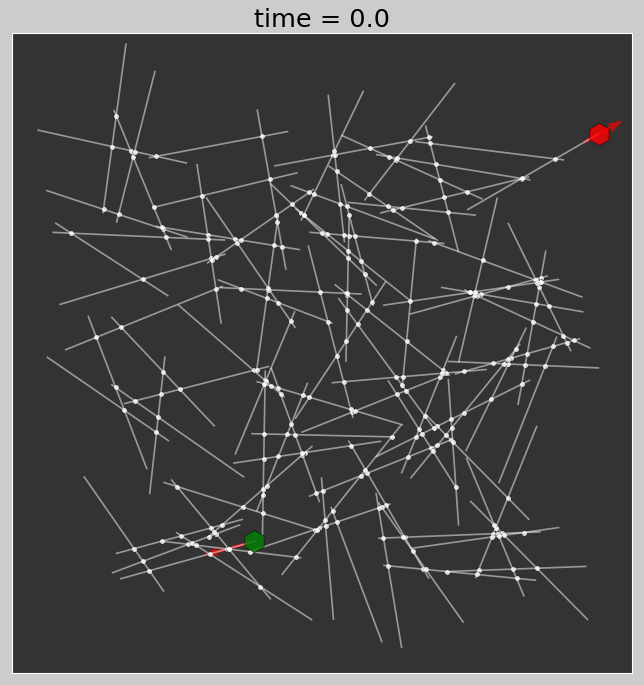
\includegraphics[width=0.7\linewidth]{figure/mpl_plot}
	\caption{}
	\label{fig:mpl_plot}
\end{figure}

\begin{figure}[h]
	\centering
	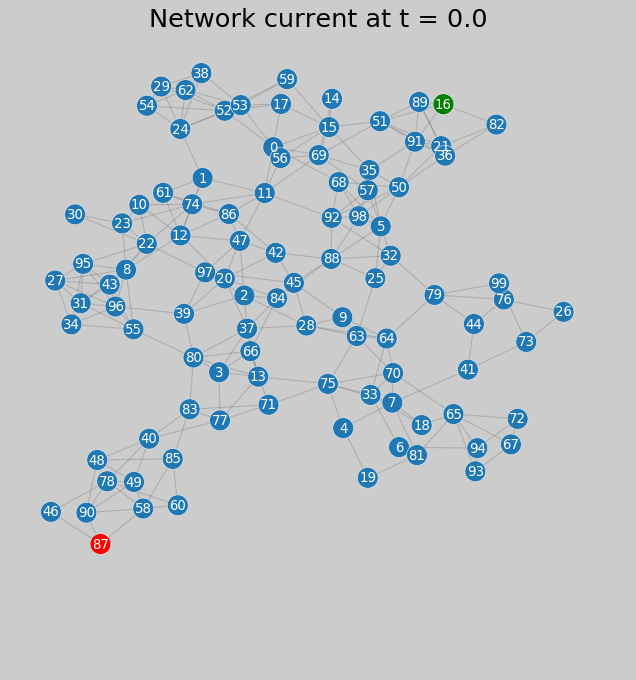
\includegraphics[width=0.8\linewidth]{figure/graph_plot}
	\caption{}
	\label{fig:graph_plot}
\end{figure}

\subsection{\label{sec:level2} Centrality}
Centrality \textbf{Put some reference here} is an important measure that helps understand the fundamental structures and connectivities of networks. Betweenness centrality of nodes and edges in networks can demonstrate .... Meanwhile, closeness centrality of nodes can be used to interpret the ..... \cite{Newman2010}.

A variation of centrality measures based on current flow model proposed by Brandes and Fleischer \cite{Brandes2005} is employed here. As the electrical dynamics in our networks fall in the class of \textbf{random walks} (not sure about here).

The betweenness centrality of a edge in the networks can be determined by:

\begin{equation}
c_{CB}(e) = \frac{\sum \limits_{s \neq t \in V}\tau_{st}(e)}{(n-1)(n-2)},
\end{equation}

where $\tau_{st}(e)$ is the current flow through edge $e$ between nodes $s$ and $t$, while $n$ stands for number of nodes in the network.

The closeness centrality of a node in this context is structured in the same way as normal closeness centrality, with distance measured based on effective resistance rather than graphical distance. Therefore it is given by:

\begin{equation}
c_{CC}(v) = \frac{n-1}{\sum \limits_{v \neq w \in V} R(v,w)}.
\end{equation}
In the context of a unit $st$-current in the network, $R(v,w)$ represents the effective resistance between nodes $v$ and $w$.



\subsection{\label{sec:level2} Transfer Entropy}

Transfer entropy is an effective metric for information transduction ...... \textbf{cite Joe here}.

\begin{equation}
T_{Y \rightarrow X} = \sum \limits_{u_n} p(u_n) \log \frac{p(x_{n+1}| x_n^{(k)}, y_n^{(l)})}{p(x_{n+1}|x_n^{(k)})}.
\end{equation}

$n$ is a time index, $u_n$ represents the state transition tuple $(x_{n+1}, x_n^{(k)}, y_n^{(l)})$, $x_n^{(k)}, y_n^{(l)}$ represent the $k$ and $l$ past values of $x$ and $y$ up to and including time $n$. \textbf{rephrase here}.

\subsection{\label{sec:level2} Modularity}
Modularity is a network metric that ..... \textbf{talk about it here} \cite{Rubinov2009}.

Recent studies in neuro-science demonstrated that modularity plays an important role in .... \textbf{talk about it here} \cite{Godwin2015}. 
 
Modularity ($Q^w$) in a weighted network can be calculated by the Louvain method \cite{Blondel2008}:
 
\begin{equation}
Q^w = \frac{1}{I^w} \sum \limits_{i,j} \left[W_{ij} - \frac{k_i^w k_j^w}{I^w} \right] \delta(m_i, m_j),
\end{equation}

in which $w_{i,j}$ is the weight of the edge between nodes $i$ and $j$, $I^w$ represents sum of all weights in the network, $k_i^w$ stands for the weighted degree of node $i$, $m_i$ is the community where node $i$ is located, and $\delta$ is the Kronecker delta function.

\section{\label{sec:level1} Results }

\subsection{\label{sec:level2} Centrality and Dynamics}

\textbf{100 nw is used here. Might have to use 700 nw for consistency.}


\paragraph{Voltage distribution}

Voltage distribution at a specific time $t$ in the network can be roughly determined by the weighted current flow betweenness centrality. As shown in fig. \ref{fig:v_lam_cent}, voltage and filament state as functions of centrality is plotted. 

\begin{itemize}
\item \textbf{Rephrase here.}
\item Two clustered groups (ON and OFF). 
\item Transition in between because of the continuity brought in by tunneling model.
\item Maybe include power consumption here as well.
\end{itemize}

\begin{figure}[h]
	\centering
	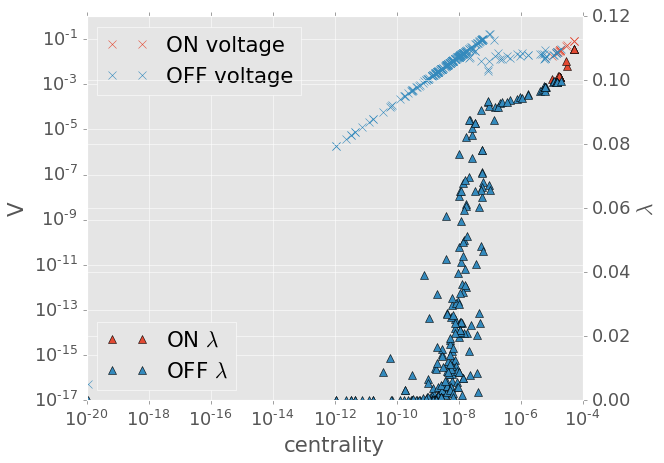
\includegraphics[width=1\linewidth]{figure/v_lam_cent}
	\caption{T=2.9, around pathway formation. crosses are voltages and triangles are filament states.}
	\label{fig:v_lam_cent}
\end{figure}

\paragraph{Current flow}

\textbf{Maybe try power dissipation of nanowire as well.}

The cumulative current flow through nanowires shows are linear relationship versus node current flow betweenness centrality. fig. \ref{fig:i_cent}.

\begin{figure}[h]
	\centering
	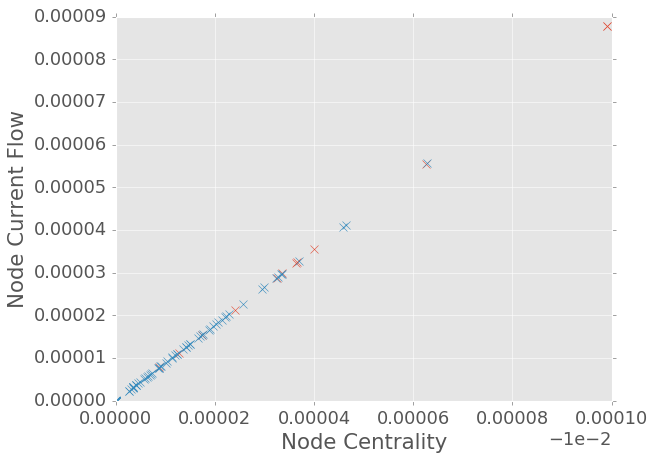
\includegraphics[width=1\linewidth]{figure/I_cent}
	\caption{Current flow on a nanowire vs node centrality}
	\label{fig:i_cent}
\end{figure}

\subsection{\label{sec:level2} Centrality and Functionality}

\paragraph{Mean communicability}
Briefly Introduce the idea of communicability. 

The communicability matrix ($M$) is generated based on $W$.... Each entry represents .... \textbf{might cite some Comm paper here}.

The row sum of $M$ can somehow interpret how communicable a node is to the rest of the network.

The plot of comm vs node closeness cent shows something .....

\begin{figure}[h]
	\centering
	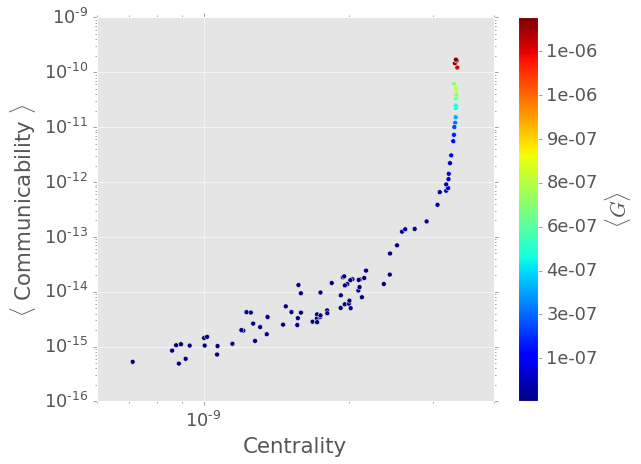
\includegraphics[width=1\linewidth]{figure/comm_cent}
	\caption{}
	\label{fig:comm_cent}
\end{figure}

\paragraph{Node Transfer Entropy}
The wire closeness centrality also shows an interesting correlation with transfer entropy. More specifically, the capabilities of taking in and giving out information. 

The transfer entropy across an edge ($e_{i,j}$) is calculated by:

\textbf{Have to write these equations in a better manner.}

\begin{equation}
TE_{i,j} = T_{V_i \rightarrow V_j}
\end{equation}

And therefore the average outward TE and inward TE of a node can be calculated by:

\begin{equation}
\langle TEout_i \rangle = \frac{\sum \limits_{i,j, A_{i,j} \neq 0} TEout}{\text{\# of edges connected to i}}
\end{equation}

With 50 repetitions of different source/target pairing (while keeping the graphical distance between them constant), TE shows a close to linear relationship with centrality as well:

\begin{figure}[h]
	\centering
	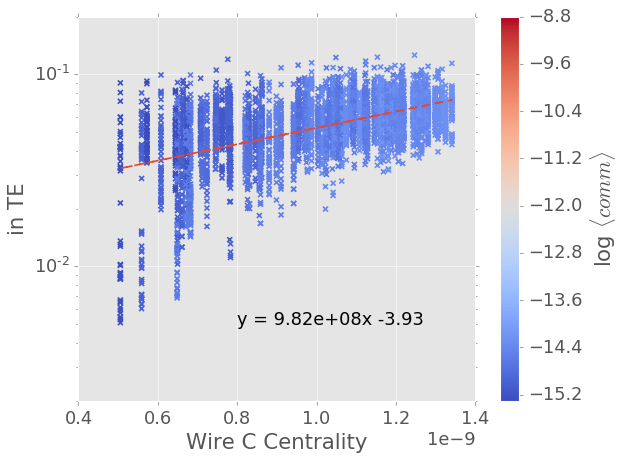
\includegraphics[width=1\linewidth]{figure/in_TE}
	\caption{}
	\label{fig:in_te}
\end{figure}

\begin{figure}[h]
	\centering
	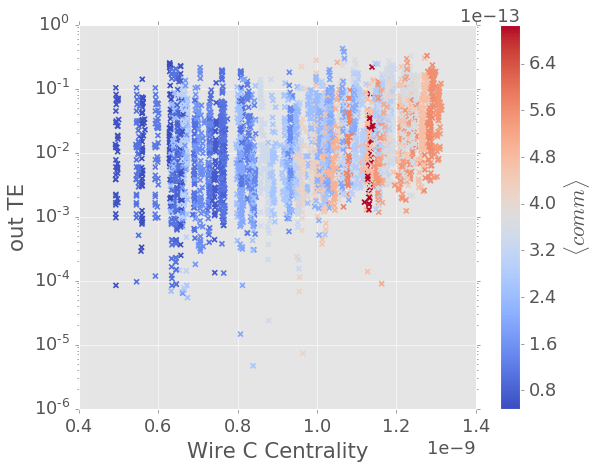
\includegraphics[width=1\linewidth]{figure/out_TE}
	\caption{}
	\label{fig:out_te}
\end{figure}


\paragraph{Node Active Information Storage}
\textbf{Not sure whether we need it here}.

\subsection{Time-series analysis}

\paragraph{$\Delta G$}

The conductance time-series of the network reflects the activation stage of the network. Specifically, $\Delta G$ can help identify the avalanche behaviors of the network.

\begin{figure}[h]
	\centering
	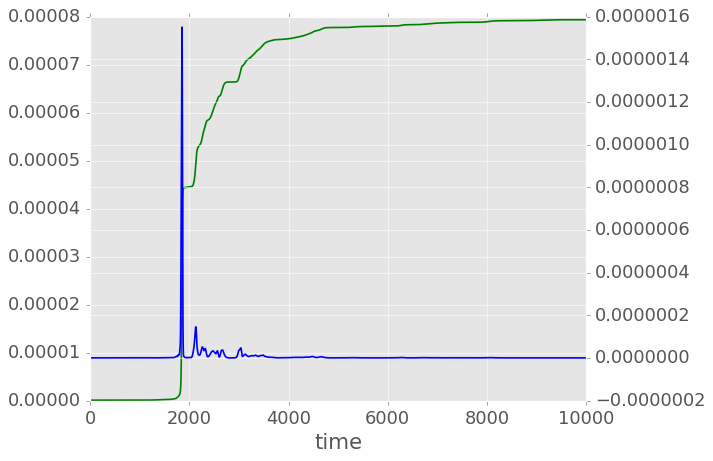
\includegraphics[width=1\linewidth]{figure/G_dG_t}
	\caption{}
	\label{fig:g_dg_t}
\end{figure}

\paragraph{TE time series}

The transfer entropy across the whole network is calculated in the same way as before. The average is taken over the whole network the time series to obtain the time series.

Plotting TE time-series together with $\Delta G$ in the same figure, the spikes of both curves coincide.

\begin{figure}[h]
	\centering
	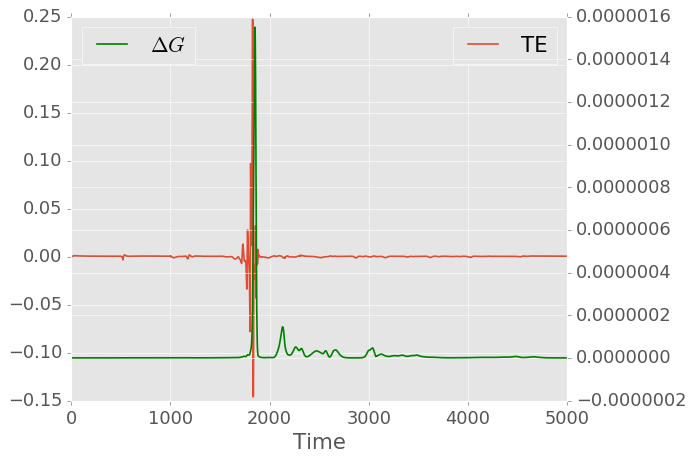
\includegraphics[width=1\linewidth]{figure/TE_dG}
	\caption{}
	\label{fig:te_dg}
\end{figure}

Different amplitude of voltage biases are applied to the network. The activation time and TE peak time in these realizations line-up pretty well.

\begin{figure}[h]
	\centering
	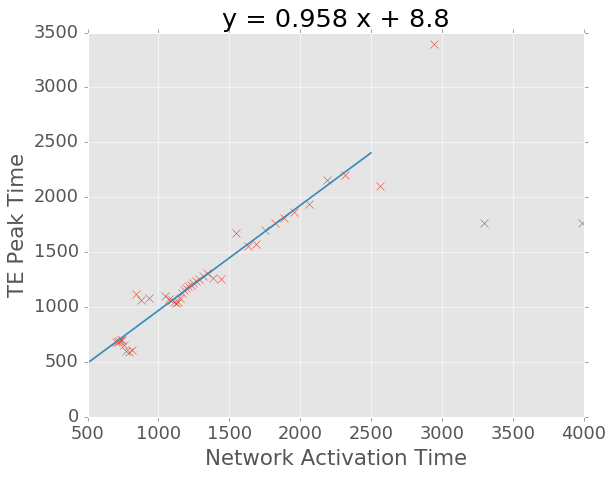
\includegraphics[width=1\linewidth]{figure/TE_act_time}
	\caption{}
	\label{fig:te_act_time}
\end{figure}


\paragraph{Modularity time series}

Modularity of the network is calculated throughout the activation. The drop of Modularity coincide with $\Delta G$ as well. 

\begin{figure}[h]
	\centering
	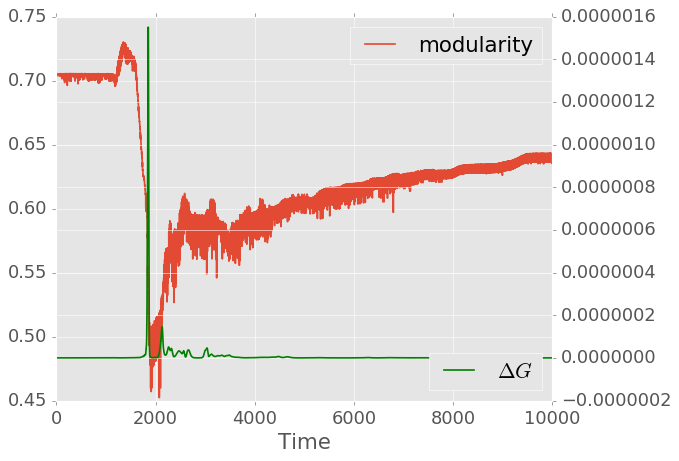
\includegraphics[width=1\linewidth]{figure/mod_dG}
	\caption{}
	\label{fig:mod_dg}
\end{figure}

\subsection{Dual task}

Pre-activate the network with Mackey-Glass signal, extract the state from different time-points. Then do a non-linear signal transform on it.

\begin{figure}[h]
	\centering
	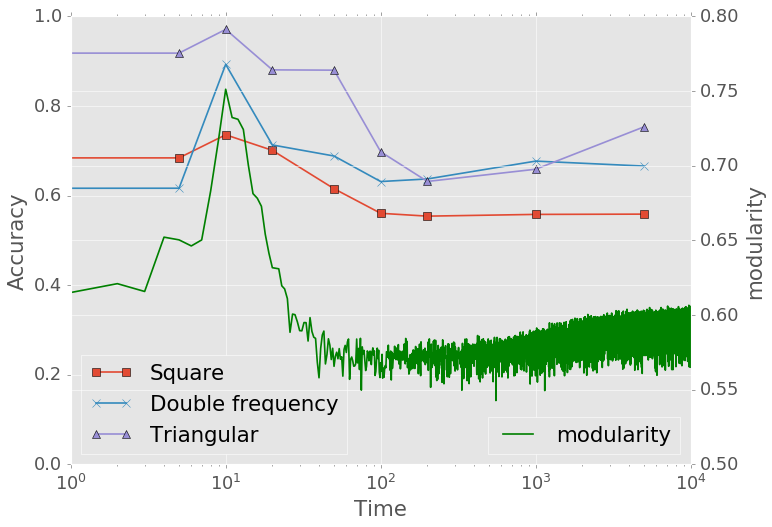
\includegraphics[width=1\linewidth]{figure/dual_task}
	\caption{}
	\label{fig:dual_task}
\end{figure}

The Guimera \textbf{cite here} plots can be displayed as follow:
 
\begin{figure}[h]
	\centering
	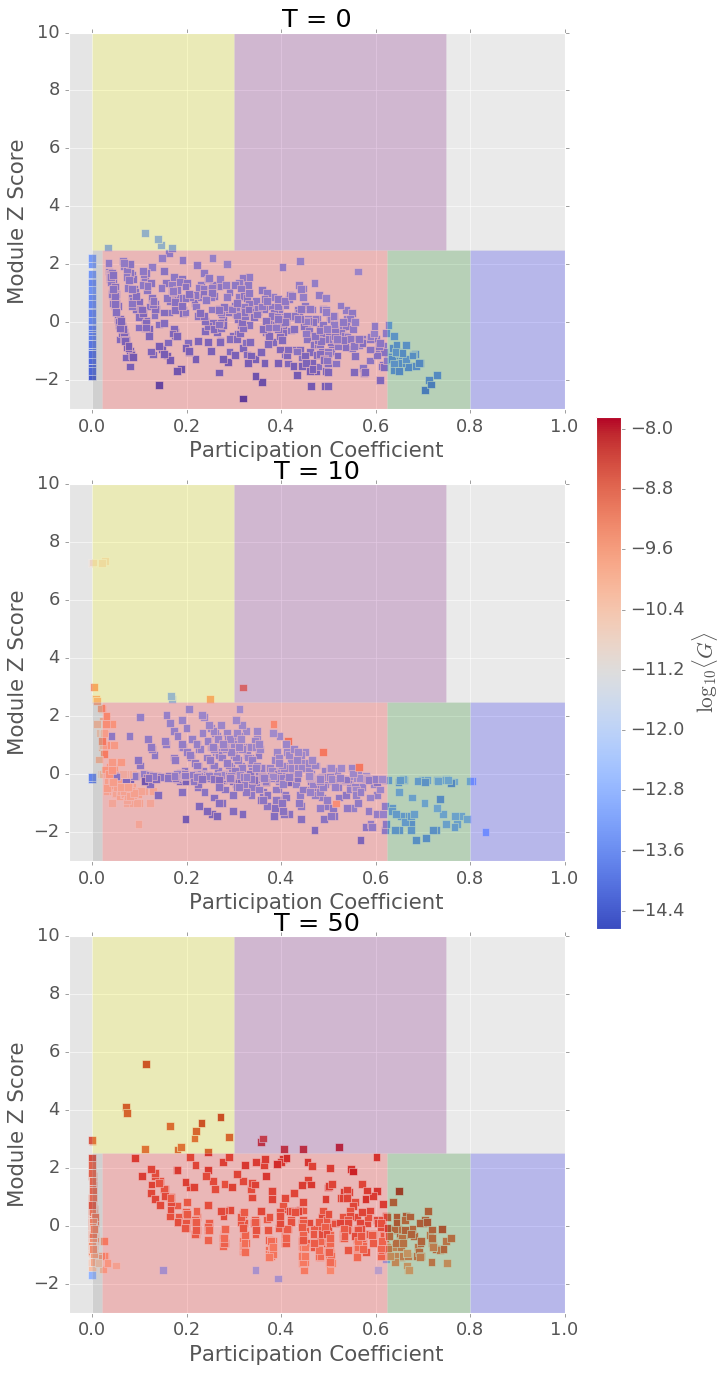
\includegraphics[width=1\linewidth]{figure/guimera_combine}
	\caption{}
	\label{fig:guimera_combine}
\end{figure}

\textbf{Have to match the color bars here.}


\newpage
\section{\label{sec:level1} Discussion}

\section{\label{sec:level1} Conclusion}








\begin{acknowledgments}
We wish to acknowledge the support of the author community in using
REV\TeX{}, offering suggestions and encouragement, testing new versions,
\dots.
\end{acknowledgments}

\appendix

\section{Appendixes}



\section{A little more on appendixes}



% The \nocite command causes all entries in a bibliography to be printed out
% whether or not they are actually referenced in the text. This is appropriate
% for the sample file to show the different styles of references, but authors
% most likely will not want to use it.
\nocite{*}



\bibliography{paper1} \label{paper1}% Produces the bibliography via BibTeX.
\bibliographystyle{apalike}

\end{document}
%
% ****** End of file apssamp.tex ******
